\documentclass[]{standalone}%
%
\usepackage{tikz, varwidth}%
\usetikzlibrary{shapes.geometric, positioning}%
%
\definecolor{TUMBlack}{cmyk}{0,0,0,1}%
\definecolor{TUMBlue}{cmyk}{1,0.43,0,0}%           Pantone 300
\definecolor{TUMBlue1}{cmyk}{1,0.57,0.12,0.7}%     Pantone 540
\definecolor{TUMBlue2}{cmyk}{1,0.54,0.04,0.19}%    Pantone 301
\definecolor{TUMBlue3}{cmyk}{0.65,0.19,0.01,0.04}% Pantone 542
\definecolor{TUMBlue4}{cmyk}{0.42,0.09,0,0}%       Pantone 283
\definecolor{TUMOrange}{cmyk}{0,0.65,0.95,0}%
\definecolor{TUMGreen}{cmyk}{0.35,0,1,0.2}%
%
\begin{document}%
%
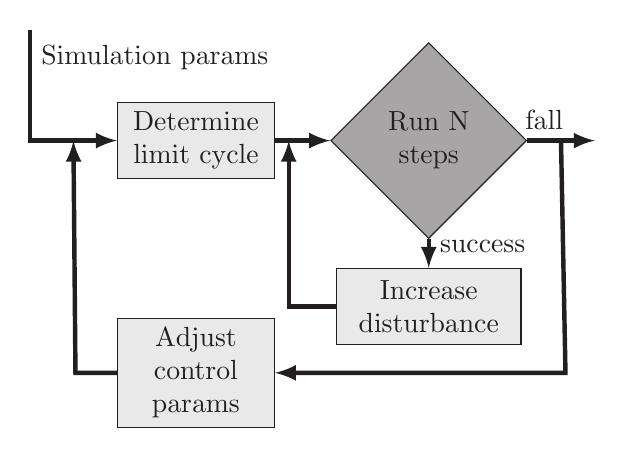
\begin{tikzpicture}[scale = 1, node distance = 6em]%
    %
    \tikzstyle{arrow} = [->, -latex, draw = TUMBlack, ultra thick, color=TUMBlack]%
    \tikzstyle{bigblock} = [rectangle, draw = TUMBlack, fill = TUMBlack!20, text width = 16em, text badly centered, text = TUMBlack, rounded corners, minimum height = 2em]%
    \tikzstyle{block} = [rectangle, draw = TUMBlack, fill = TUMBlack!10, text width = 5em, text badly centered, text = TUMBlack, minimum height = 2.75em]%
    \tikzstyle{decision} = [diamond, draw = TUMBlack, fill = TUMBlack!40, text width = 5em, text badly centered, text = TUMBlack, node distance = 1.5cm, inner sep = 0pt]%
    % 
    \coordinate [] (start) {};%
    \coordinate [above = 4em of start] (A) {};%
    \node [block, right of = start] (limit-cycle) {Determine limit cycle};%
    \node [decision, right = 2em of limit-cycle] (steps) {Run N steps};%
    \node [block, below of = steps, text width = 6em] (increase-disturbance) {Increase disturbance};%
    \node [block, below = 5em of limit-cycle] (adjust-control-params) {Adjust control params};%
    %
    \path [arrow] (A) -- (start.west) node [right, near start, text = TUMBlack] {Simulation params} -- (limit-cycle) node [midway] (H) {};%
    \path [arrow] (limit-cycle) -- (steps) node [near start] (C) {};%
    \coordinate [right of = steps] (B);%
    \path [arrow] (steps) -- (B) node [above, near start, text = TUMBlack] {fall} node [midway] (E) {};%
    \path [arrow] (steps) -- (increase-disturbance) node [right, near start, text = TUMBlack] {success};%
    %
    \coordinate [below of = C] (D);%
    \path [arrow] (increase-disturbance) -- (D) -- (C.center);%
    %
    \coordinate [right = 10.5em of adjust-control-params] (F);%
    \path [arrow] (E.center) -- (F) -- (adjust-control-params);%
    %
    \coordinate [left = 1.5em of adjust-control-params] (G);%
    \path [arrow] (adjust-control-params) -- (G) -- (H.center);%
    % 
\end{tikzpicture}%
%
\end{document}%
%